\section{Exactness is not accuracy}
\label{sec:numerics}

Before attributing the learning probes to operator structure, the paper checks
whether this implementation has a floating-point accuracy advantage.
It does not on the finite precision grid below. The grid supplies no evidence
for that explanation; it is not a universal comparison of
sparse and dense factorization accuracy.

\paragraph{No robust win in either direction.}
Scored on the pattern against a 64-bit oracle and swept over conditioning
(Table~\ref{tab:precision}), the selected inverse and a dense SPD solve at
equal 32-bit floating-point (fp32) precision stay within small constant
factors of each other across
structures and $\kappa$: the error ratio ranges from $0.34$ to $1.95$ with no
consistent direction (at the highest-$\kappa$ grid cell the dense solve is in
fact the more accurate, by more than $2.8\times$). An initial reading of roughly $1.9\times$
on trees, growing with $\kappa$, on ill-scaled random matrices turned out,
over enough seeds (16 for the ordering study), to be a ratio-of-medians
artifact, and most of the modest, heavy-tailed median gap is an
elimination-ordering effect: a dense Cholesky run in the kernel's own
leaf-first order has comparable accuracy. No consistent accuracy edge appears
on this grid. The 16-seed ordering diagnostic is recorded in
\url{paper/attainability/figures/data/precision_compare_orders.txt}.

\begin{table}[htbp]
  \centering
  \caption{Selected inverse vs.\ dense Cholesky at equal fp32 precision,
  scored on-pattern against an fp64 oracle. Entries are medians over four
  seeds per cell; the ratio is the median per-seed dense/selected-inverse
  error ratio. Displayed errors and ratios are rounded conservatively against
  the selected-inverse arm. Data:
  \url{paper/attainability/figures/data/precision_tree.csv} and
  \url{paper/attainability/figures/data/precision_grid.csv}.}
  \label{tab:precision}
  \begin{tabular}{lcccc}
    \toprule
    structure & $\kappa$ & selected-inverse error & dense error & ratio \\
    \midrule
    tree ($n{=}127$) & $6.0\mathrm{e}{+1}$ & $1.6\mathrm{e}{-7}$ & $2.0\mathrm{e}{-7}$ & $1.32$ \\
    tree ($n{=}127$) & $5.8\mathrm{e}{+3}$ & $6.2\mathrm{e}{-6}$ & $1.1\mathrm{e}{-5}$ & $1.95$ \\
    tree ($n{=}127$) & $2.9\mathrm{e}{+5}$ & $4.2\mathrm{e}{-4}$ & $4.5\mathrm{e}{-4}$ & $1.64$ \\
    grid ($8{\times}8$) & $1.8\mathrm{e}{+1}$ & $1.7\mathrm{e}{-7}$ & $1.4\mathrm{e}{-7}$ & $0.88$ \\
    grid ($8{\times}8$) & $1.7\mathrm{e}{+3}$ & $3.2\mathrm{e}{-6}$ & $3.4\mathrm{e}{-6}$ & $1.10$ \\
    grid ($8{\times}8$) & $1.7\mathrm{e}{+5}$ & $8.5\mathrm{e}{-4}$ & $2.7\mathrm{e}{-4}$ & $0.34$ \\
    \bottomrule
  \end{tabular}
\end{table}

\paragraph{What exactness does give: a sparse-structured global operator.}
The edge is not a more accurate rounded number; it is that the operator is
algebraically exact, global, and sparse-structured. That structure is what
makes the operator usable as a layer:
Figure~\ref{fig:scaling} shows forward timings consistent with the chain's
$\bigO(n)$ operation count, with the measured dense crossover, and
forward-plus-backward Gaussian Markov random field (GMRF) training timings
consistent with linear tree work
where dense autograd is $\bigO(N^3)$. The cost still grows with problem size,
linearly on the chain shown here; it does not acquire an iteration count
proportional to graph distance. That is the distinction the next two sections
exploit.

\providecommand{\scalingfigurewidth}{0.92\textwidth}
\begin{figure}[htbp]
  \centering
  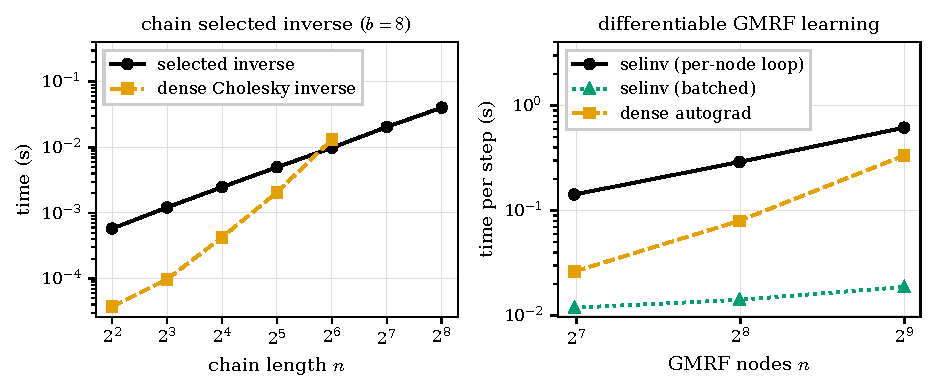
\includegraphics[width=\scalingfigurewidth]{figures/scaling.pdf}
  \caption{Scaling diagnostics on a central processing unit (CPU). Left:
  forward time for a 64-bit floating-point (fp64) block-chain
  selected inverse ($b=8$) and a dense Cholesky inverse, using the median of
  three seed-wise timing medians. Right: forward-plus-backward time per
  differentiable tree Gaussian Markov random field (GMRF) training step and
  dense autograd. Timings depend on the basic linear algebra subprograms
  (BLAS) library and device; no graphics processing unit (GPU) claim is made.
  Data:
  \href{bench_results.csv}{\texttt{bench\_results.csv}}
  and
  \href{paper/attainability/figures/data/gmrf_scaling.csv}{\texttt{gmrf\_scaling.csv}}.}
  \label{fig:scaling}
\end{figure}
